\begin{figure}[htbp]
			\centering
			\resizebox{\textwidth}{!}{%
				\begin{tikzpicture}[
					scale=0.95,
					>=latex,
					trave/.style={line width=2pt},
					forza/.style={black, line width=1pt},
					diagT/.style={black, line width=0.8pt},
					diagM/.style={black, line width=0.8pt},
					hatch/.style={gray!50, line width=0.3pt},
					quota/.style={black, line width=0.4pt},
					fibre/.style={gray!70, line width=0.3pt},
					]
					
					% ── Parametri dei vincoli (convenzione C06/C07) ──
					\def\tw{0.15}    \def\thR{0.28}   \def\rn{0.06}
					\def\rw{0.05}    \def\bw{0.09}    \def\gw{0.22}
					\def\hh{0.10}
					
					% ── Geometria del problema ──
					\def\Lell{4}                 % lunghezza trave ℓ
					\def\aa{1.5}                 % distanza AC = a
					\def\bb{2.5}                 % distanza CB = b
					\def\yq{-0.80}               % y delle quote sotto la trave
					\def\yconcio{-0.80}          % y del concio di legenda
					\def\ylab{-3.30}             % y delle etichette di pannello (a, b, c)
					\def\LT{0.30}    % semi-lunghezza della freccia di T (lunghezza totale = 2*LT)
					
					% =========================================================
					% PANNELLO (a) — Schema statico e legenda del concio
					% =========================================================
					\begin{scope}[xshift=0cm]
						
						% ── Trave ──
						\draw[trave] (0,0) -- (\Lell,0);
						
						% ── Fibra inferiore (tratteggio sotto la trave) ──
						\draw[fibre, dashed] (0, -0.1) -- (\Lell, -0.1);
						
						% ── Cerniera in A ──
						\draw[thick] (0,0) -- (-\tw,-\thR) -- (\tw,-\thR) -- cycle;
						\draw[thick] (-\gw,-\thR) -- (\gw,-\thR);
						\foreach \x in {-0.16,-0.08,0,0.08,0.16}
						\draw[thin] (\x,-\thR) -- ++(-0.07,-\hh);
						
						% ── Carrello verticale in B ──
						\draw[thick] (\Lell,0) -- (\Lell-\tw,-\thR) -- (\Lell+\tw,-\thR) -- cycle;
						\draw[thick] (\Lell-\bw,-\thR-\rw-0.01) circle (\rw);
						\draw[thick] (\Lell+\bw,-\thR-\rw-0.01) circle (\rw);
						\draw[thick] (\Lell-\gw,-\thR-2*\rw-0.04) -- (\Lell+\gw,-\thR-2*\rw-0.04);
						\foreach \x in {-0.16,-0.08,0,0.08,0.16}
						\draw[thin] (\Lell+\x,-\thR-2*\rw-0.04) -- ++(-0.07,-\hh);
						
						% ── Anellini ──
						\draw[thick, fill=white] (0,0) circle (\rn);
						\draw[thick, fill=white] (\Lell,0) circle (\rn);
						
						% ── Etichette A, B, C ──
						\node[above left=-2pt,  font=\small] at (0,0)       {$A$};
						\node[above right=-2pt, font=\small] at (\Lell,0)   {$B$};
						\node[below,            font=\small] at (\aa,0.05)  {$C$};
						
						% ── Forza concentrata F in C (verticale, verso il basso) ──
						\def\Lf{0.80}
						% tacca verticale che marca il punto C sull'asse
						\draw[forza] (\aa, -0.10) -- (\aa, 0.10);
						% freccia: parte sopra la trave, scende verso il basso, punta sulla trave
						\draw[->, forza] (\aa, 0.10 + \Lf) -- (\aa, 0.10);
						% etichetta sopra la freccia
						\node[right, font=\small] at (\aa+0.05, 0.10 + 0.5*\Lf) {$F$};
						
						% ── Quote a e b sopra la trave, al di sopra della coda di F ──
						\def\yqs{1.20}    % y della linea di quotatura (sopra la coda di F a y=0.90)
						\draw[<->, quota] (0,\yqs) -- (\aa,\yqs);
						\draw[<->, quota] (\aa,\yqs) -- (\Lell,\yqs);
						\draw[quota] (0,\yqs+0.07) -- (0,\yqs-0.07);
						\draw[quota] (\aa,\yqs+0.07) -- (\aa,\yqs-0.07);
						\draw[quota] (\Lell,\yqs+0.07) -- (\Lell,\yqs-0.07);
						\node[below, font=\small] at ({0.5*\aa}, \yqs-0.04)        {$a$};
						\node[below, font=\small] at ({0.5*(\aa+\Lell)}, \yqs-0.04) {$b$};
						
						
						% ── Concio di legenda (sotto le quote) ──
						% concio orientato verticalmente: lato corto parallelo alla trave
						\def\Lc{0.40}       % larghezza del concio (lato corto, // alla trave)
						\def\Hc{0.90}       % altezza del concio (lato lungo, ⊥ alla trave)
						\pgfmathsetmacro{\xc}{\aa + 1.0}             % ascissa sx del concio
						\pgfmathsetmacro{\xcd}{\xc + \Lc}            % ascissa dx del concio
						\pgfmathsetmacro{\yct}{\yconcio + 0.5*\Hc}   % y bordo superiore
						\pgfmathsetmacro{\ycb}{\yconcio - 0.5*\Hc}   % y bordo inferiore
						
						% Corpo del concio (rettangolo verticale)
						\draw[thick] (\xc, \ycb) rectangle (\xcd, \yct);
						
						% Fibra inferiore del concio
						% (linea tratteggiata orizzontale appena sopra il bordo inferiore)
						\draw[fibre, dashed] (\xc, \ycb - 0.05) -- (\xcd, \ycb - 0.05);
						
						
						% Taglio positivo T+ (convenzione: orario sul concio)
						% Faccia sinistra: freccia verso il basso (T positivo entra dal basso)
						\draw[<-, forza] (\xc - 0.10, \yconcio + \LT) -- (\xc - 0.10, \yconcio - \LT);
						%				% Faccia destra: freccia verso l'alto (T positivo esce verso l'alto)
						\draw[<-, forza] (\xc + \Lc + 0.10, \yconcio - \LT) -- (\xc + \Lc + 0.10, \yconcio + \LT);
						% etichetta T
						%\node[font=\footnotesize] at (\xc - 0.32, \yconcio) {$T$};
						\node[font=\small] at (\xc + \Lc + 0.32, \yconcio) {$T$};
						
						% ── Momento positivo M+ destro (concavità verso il concio, oltre l'etichetta T) ──
						\def\RarcoM{0.40}      % raggio dell'arco di M (quasi metà altezza del concio)
						\def\dM{0.20}          % distanza orizzontale dell'arco dal bordo destro del concio
						% (deve essere > posizione della freccia T + larghezza etichetta T)
						
						% Centro dell'arco: spostato a destra del concio, allineato verticalmente al centro
						\pgfmathsetmacro{\xMc}{\xcd + \dM}
						\pgfmathsetmacro{\yMc}{\yconcio}
						
						% Arco: parte in alto (90°), curva a destra (passando per 0°), arriva in basso (-90°)
						% Convessità a destra = arco aperto a sinistra = concavità verso il concio
						\draw[<-, forza]
						(\xMc, \yMc + \RarcoM)         % punto di partenza in alto
						arc (90:-90:\RarcoM);          % arco da 90° a -90° = semicerchio destro
						
						% Etichetta M a destra dell'arco
						\node[right, font=\small] at (\xMc + \RarcoM-0.05, \yMc) {$M$};
						
						% ── Momento positivo M+ sinistro (concavità verso il concio) ──
						% (stessi parametri \RarcoM e \dM del momento destro per simmetria)
						
						% Centro dell'arco: spostato a sinistra del concio, allineato verticalmente al centro
						\pgfmathsetmacro{\xMcL}{\xc - \dM}
						\pgfmathsetmacro{\yMcL}{\yconcio}
						
						% Arco: parte in alto (90°), curva a sinistra (passando per 180°), arriva in basso (270°)
						% Convessità a sinistra = arco aperto a destra = concavità verso il concio
						\draw[<-, forza]
						(\xMcL, \yMcL + \RarcoM)         % punto di partenza in alto
						arc (90:270:\RarcoM);            % arco da 90° a 270° = semicerchio sinistro
						
						
						% Etichetta pannello
						\node[font=\small] at (0.20*\Lell, \ylab/2) {(a)};
						
					\end{scope}
					
					% =========================================================
					% PANNELLO (b) — Diagramma di T(z)
					% =========================================================
					\begin{scope}[xshift=6cm]
						
						% ── Trave (clone) ──
						\draw[trave] (0,0) -- (\Lell,0);
						
						% ── Vincoli (clone esatto dal pannello a) ──
						\draw[thick] (0,0) -- (-\tw,-\thR) -- (\tw,-\thR) -- cycle;
						\draw[thick] (-\gw,-\thR) -- (\gw,-\thR);
						\foreach \x in {-0.16,-0.08,0,0.08,0.16}
						\draw[thin] (\x,-\thR) -- ++(-0.07,-\hh);
						\draw[thick] (\Lell,0) -- (\Lell-\tw,-\thR) -- (\Lell+\tw,-\thR) -- cycle;
						\draw[thick] (\Lell-\bw,-\thR-\rw-0.01) circle (\rw);
						\draw[thick] (\Lell+\bw,-\thR-\rw-0.01) circle (\rw);
						\draw[thick] (\Lell-\gw,-\thR-2*\rw-0.04) -- (\Lell+\gw,-\thR-2*\rw-0.04);
						\foreach \x in {-0.16,-0.08,0,0.08,0.16}
						\draw[thin] (\Lell+\x,-\thR-2*\rw-0.04) -- ++(-0.07,-\hh);
						\draw[thick, fill=white] (0,0) circle (\rn);
						\draw[thick, fill=white] (\Lell,0) circle (\rn);
						
						% ── Etichette A, B, C ──
						\node[above left=-2pt,  font=\small] at (0,0)       {$A$};
						\node[above right=-2pt, font=\small] at (\Lell,0)   {$B$};
						\node[below left,   font=\small] at (\aa,0.05)  {$C$};
						
						% ── Diagramma T(z) ──
						% Scala 1 F = \sT unità di figura
						% Convenzione: T positivo sopra, T negativo sotto
						\def\sT{1.40}
						\pgfmathsetmacro{\Tpos}{(\bb/\Lell)*\sT}    % T(AC) = +Fb/ℓ
						\pgfmathsetmacro{\Tneg}{-(\aa/\Lell)*\sT}   % T(CB) = -Fa/ℓ
						
						% Hatching verticale nelle due aree
						% Tratto AC: dal'asse al livello Tpos (sopra)
						\foreach \x in {0.10, 0.30, ..., 1.40} {
							\draw[hatch] (\x, 0) -- (\x, \Tpos);
						}
						% Tratto CB: dall'asse al livello Tneg (sotto)
						\foreach \x in {1.60, 1.80, ..., 3.90} {
							\draw[hatch] (\x, 0) -- (\x, \Tneg);
						}
						
						% Bordo del diagramma (linea spessa nera)
						% Verticale in A, orizzontale fino a C, verticale del salto in C,
						% orizzontale fino a B, verticale di chiusura in B
						\draw[diagT]
						(0, 0) -- (0, \Tpos)              % verticale in A
						-- (\aa, \Tpos)                   % orizzontale tratto AC
						-- (\aa, \Tneg)                   % salto verticale in C
						-- (\Lell, \Tneg)                 % orizzontale tratto CB
						-- (\Lell, 0);                    % verticale in B
						
						% Segno "+" cerchiato (area positiva, tratto AC)
						\node[circle, draw, fill=white, thick,	minimum size=10pt, inner sep=0pt, font=\large]	at (0.5*\aa, 0.5*\Tpos) {$+$};
						
						% Segno "-" cerchiato (area negativa, tratto CB)
						\node[circle, draw, fill=white, thick,	minimum size=10pt, inner sep=0pt, font=\large]	at (\aa + 0.5*\bb, 0.5*\Tneg) {$-$};
						
						% Etichette dei valori notevoli
						\node[below left, font=\small] at (0, \Tpos)   {$\tfrac{Fb}{\ell}$};
						\node[right, font=\small] at (\Lell, \Tneg) {$\tfrac{Fa}{\ell}$};
						
						% Etichetta pannello
						\node[font=\small] at (0.20*\Lell, \ylab/2) {(b)};
						
					\end{scope}
					
					% =========================================================
					% PANNELLO (c) — Diagramma di M(z)
					% =========================================================
					\begin{scope}[xshift=12cm]
						
						% ── Trave (clone) ──
						\draw[trave] (0,0) -- (\Lell,0);
						
						% ── Vincoli (clone esatto dal pannello a) ──
						\draw[thick] (0,0) -- (-\tw,-\thR) -- (\tw,-\thR) -- cycle;
						\draw[thick] (-\gw,-\thR) -- (\gw,-\thR);
						\foreach \x in {-0.16,-0.08,0,0.08,0.16}
						\draw[thin] (\x,-\thR) -- ++(-0.07,-\hh);
						\draw[thick] (\Lell,0) -- (\Lell-\tw,-\thR) -- (\Lell+\tw,-\thR) -- cycle;
						\draw[thick] (\Lell-\bw,-\thR-\rw-0.01) circle (\rw);
						\draw[thick] (\Lell+\bw,-\thR-\rw-0.01) circle (\rw);
						\draw[thick] (\Lell-\gw,-\thR-2*\rw-0.04) -- (\Lell+\gw,-\thR-2*\rw-0.04);
						\foreach \x in {-0.16,-0.08,0,0.08,0.16}
						\draw[thin] (\Lell+\x,-\thR-2*\rw-0.04) -- ++(-0.07,-\hh);
						\draw[thick, fill=white] (0,0) circle (\rn);
						\draw[thick, fill=white] (\Lell,0) circle (\rn);
						
						% ── Etichette A, B, C ──
						\node[above left=-2pt,  font=\small] at (0,0)       {$A$};
						\node[above right=-2pt, font=\small] at (\Lell,0)   {$B$};
						\node[above,            font=\small] at (\aa,0.05)  {$C$};
						
						% ── Diagramma M(z) ──
						% Scala 1 F = \sM unità di figura
						% Convenzione: M positivo SOTTO l'asse (fibre tese inferiori)
						\def\sM{0.80}
						\pgfmathsetmacro{\Mmax}{-(\aa*\bb/\Lell)*\sM}    % M(C) = -Fab/ℓ (negativo perché sotto)
						
						% Hatching verticale dell'area (linee dall'asse al diagramma)
						% Tratto AC: M(z) = (Fb/ℓ) z, lineare crescente in modulo
						\foreach \x in {0.20, 0.40, ..., 1.40} {
							\pgfmathsetmacro{\h}{(\bb/\Lell)*\x*(-\sM)}
							\draw[hatch] (\x, 0) -- (\x, \h);
						}
						% Tratto CB: M(z) = (Fa/ℓ)(ℓ-z), lineare decrescente in modulo
						\foreach \x in {1.60, 1.80, ..., 3.80} {
							\pgfmathsetmacro{\h}{(\aa/\Lell)*(\Lell-\x)*(-\sM)}
							\draw[hatch] (\x, 0) -- (\x, \h);
						}
						
						% Bordo del diagramma (linea spessa nera)
						% Triangolo: da A (0,0) a C (a, Mmax) a B (ℓ, 0)
						\draw[diagM] (0, 0) -- (\aa, \Mmax) -- (\Lell, 0);
						
						% Etichetta del valore notevole in C
						\node[below, font=\small] at (\aa, \Mmax-0.04) {$\tfrac{Fab}{\ell}$};
						
						% Etichetta pannello
						\node[font=\small] at (0.2*\Lell, \ylab/2) {(c)};
					\end{scope}
					
				\end{tikzpicture}
			}
			\caption{Trave appoggiata con forza concentrata $F$ in $C$:
				(a)~schema strutturale e, nel riquadro, convenzioni di segno
				per $T$ (positivo orario sul concio) e $M$ (positivo per
				fibre inferiori tese);
				(b)~diagramma del taglio $T(z)$, uniforme a tratti con salto
				$-F$ in $C$;
				(c)~diagramma del momento flettente $M(z)$, lineare a tratti
				con massimo $Fab/\ell$ in $C$.}
			\label{fig:stat_trasv_iso_00}
		\end{figure}
